\section{Implementacion}
\begin{frame}{Implementacion}

\end{frame}

\begin{frame}{}
  \begin{columns}[c] % [c] centra verticalmente
    \column{0.5\textwidth}
      \centering
      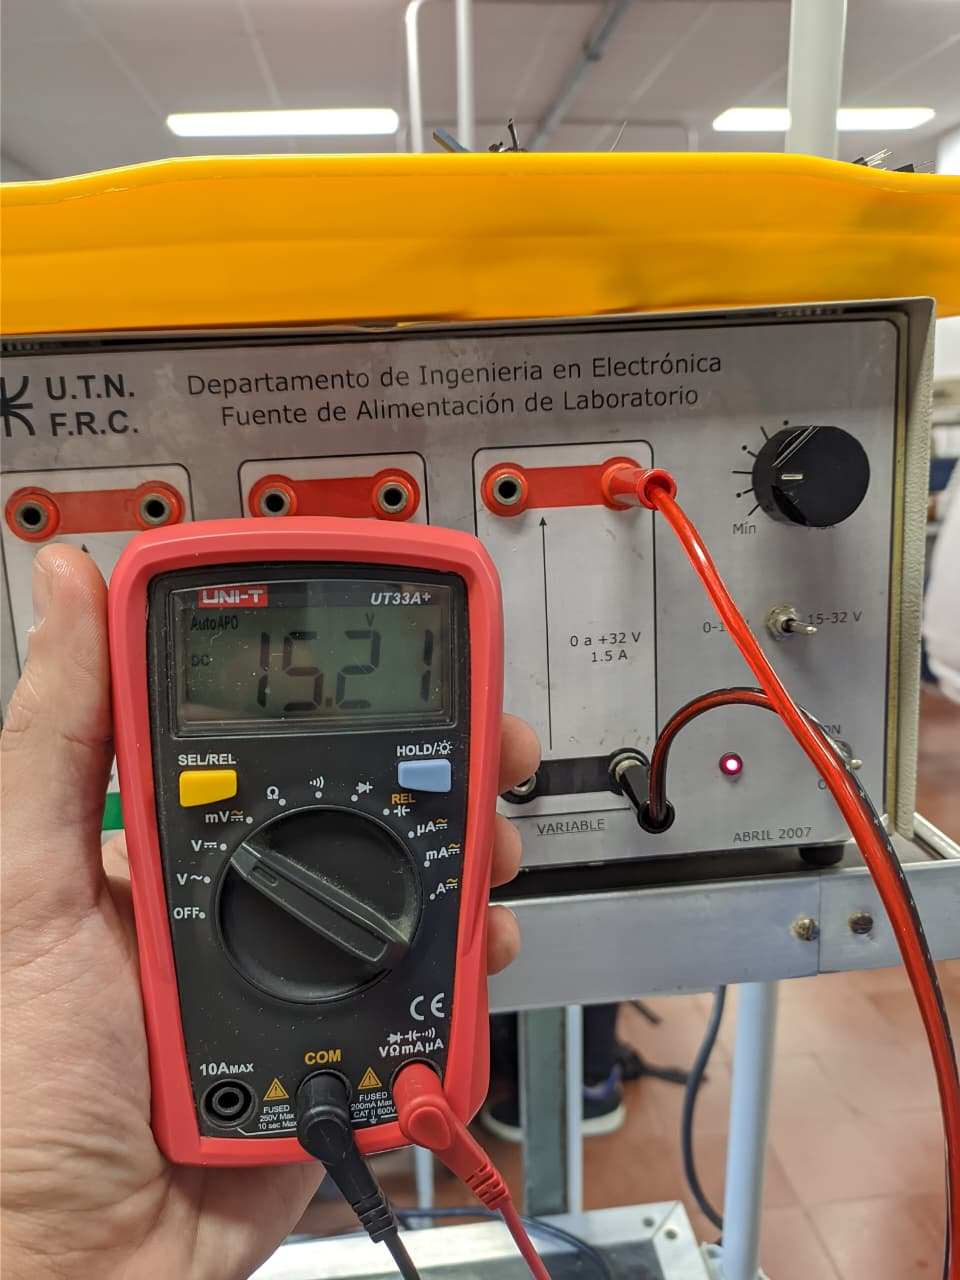
\includegraphics[width=\linewidth]{pictures/VCC.jpeg}

    \column{0.5\textwidth}
      \justifying
        Lo primero que se realiza al energizar el circuito es tomar mediciones de las caidas de tension. como se puede
        apreciar en la foto, esa es la tension de alimentacion VCC. 
      
  \end{columns}
\end{frame}

\begin{frame}{}
  \begin{table}[H]
    \centering
    \caption{Valores medidos y resistencias asociadas}
    \begin{tabular}{lcc}
    \toprule
    \textbf{Parametro} & \textbf{Tensión [V]} & \textbf{Resistencia [\(\Omega\)]} \\
    \midrule
    $V_{CC}$ & $15.21$ & -- \\
    $V_{RC}$ & $9.35$  & $2.18\,k$ \\
    $V_{CB}$ & $4.226$ & -- \\
    $V_{RE}$ & $4.26$  & $217$ \\
    $V_{R1}$ & $1.54$  & $11.96\,k$ \\
    $V_{R2}$ & $13.64$ & $99.7\,k$ \\
    \bottomrule
    \end{tabular}
  \end{table}
\end{frame}


\begin{frame}{}

  \begin{block}{Ecuaciones de referencia}
    \[
      I_{CQ} = \frac{V_{CC} - V_{BB}}{R_C + (R_C \parallel R_L) - \tfrac{R_B}{\beta}}
    \]
    \[
      V_{BB} = V_{CC}\cdot \frac{R_1}{R_1 + R_2}
      \qquad\qquad
      R_B = R_1 \parallel R_2
    \]
  \end{block}

  \begin{block}{Valores calculados}
    \[
      V_{BB} = 1.629 \,\text{V}
      \qquad
      R_B = 10\,678.95 \,\Omega
      \qquad
      I_{CQ} = 4.179 \,\text{mA}
    \]
  \end{block}

\end{frame}


\begin{frame}{}

  \begin{table}[H]
  \centering
  \begin{tabular}{lccc}
    \toprule
    \textbf{Parámetro} & \textbf{Analítico} & \textbf{±10\% del analítico} & \textbf{Calculado} \\
    \midrule
    $I_{CQ}$  & $4.121\,\text{mA}$ & $[3.709\,;\,4.533]\,\text{mA}$ & $4.179\,\text{mA}$ \\
    $V_{CBQ}$ & $4.53\,\text{V}$   & $[4.077\,;\,4.983]\,\text{V}$  & $4.226\,\text{V}$ \\
    \bottomrule
  \end{tabular}
  \end{table}

  \vspace{1em}

  \begin{block}{Observación}
    Los valores calculados se ubican dentro del rango de tolerancia del
    $\pm 10\%$ respecto de los analíticos, lo que confirma la validez del
    procedimiento experimental.
  \end{block}

\end{frame}




\begin{frame}{Parámetros hibridos}
    \begin{columns}[t]
      \column{0.48\textwidth}
      \begin{block}{Impedancia de entrada $Z_i$}
        \[
          i_i = \frac{V_s - V_i}{R_s}
          \qquad
          Z_i = \frac{V_i}{i_i}
        \]
      \end{block}
    
      \begin{block}{Ganancia de tensión $A_v$}
        \[
          A_v = \frac{V_o}{V_i}
        \]
      \end{block}
    
      \column{0.48\textwidth}
      \begin{block}{Ganancia de corriente $A_i$}
        \[
          A_i = \frac{i_o}{i_i}
          = \frac{\tfrac{V_o}{R_L}}{\tfrac{V_s - V_i}{R_s}}
        \]
      \end{block}
    
      \begin{block}{Impedancia de salida $Z_o$}
        \[
          i_o = \frac{V_s - V_o}{R_s}
          \qquad
          Z_o = \frac{V_o}{i_o}
        \]
      \end{block}
    \end{columns}

\end{frame}





\begin{frame}{}
\begin{figure}
  \centering
  \begin{subfigure}[t]{0.65\linewidth}
    \centering
    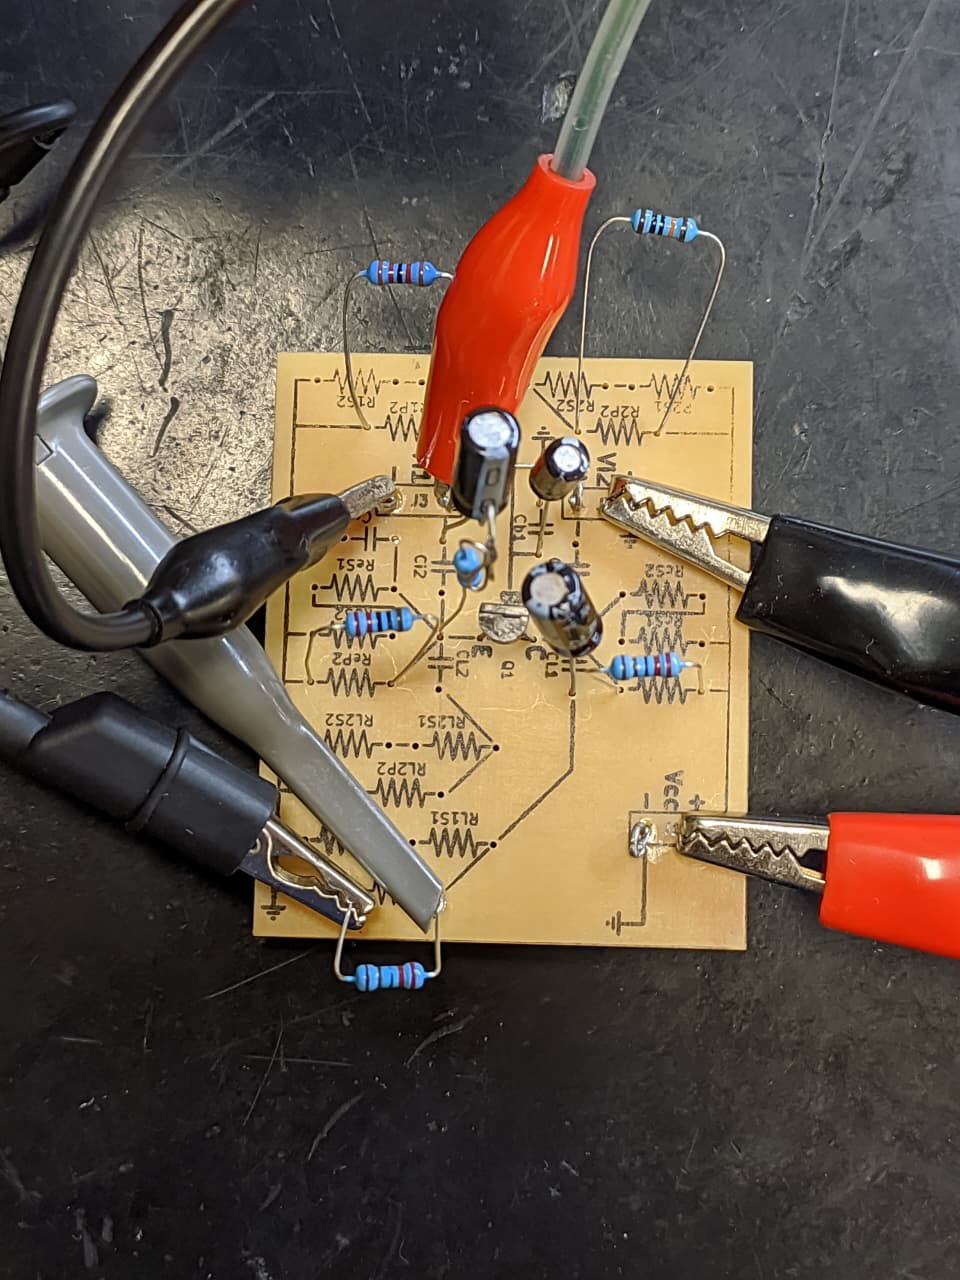
\includegraphics[height=0.65\textheight]{pictures/Placa_Zi.jpeg}
    \caption{Placa montada para medir $Z_i$.}
  \end{subfigure}\hfill
  \begin{subfigure}[t]{0.35\linewidth}
    \centering
    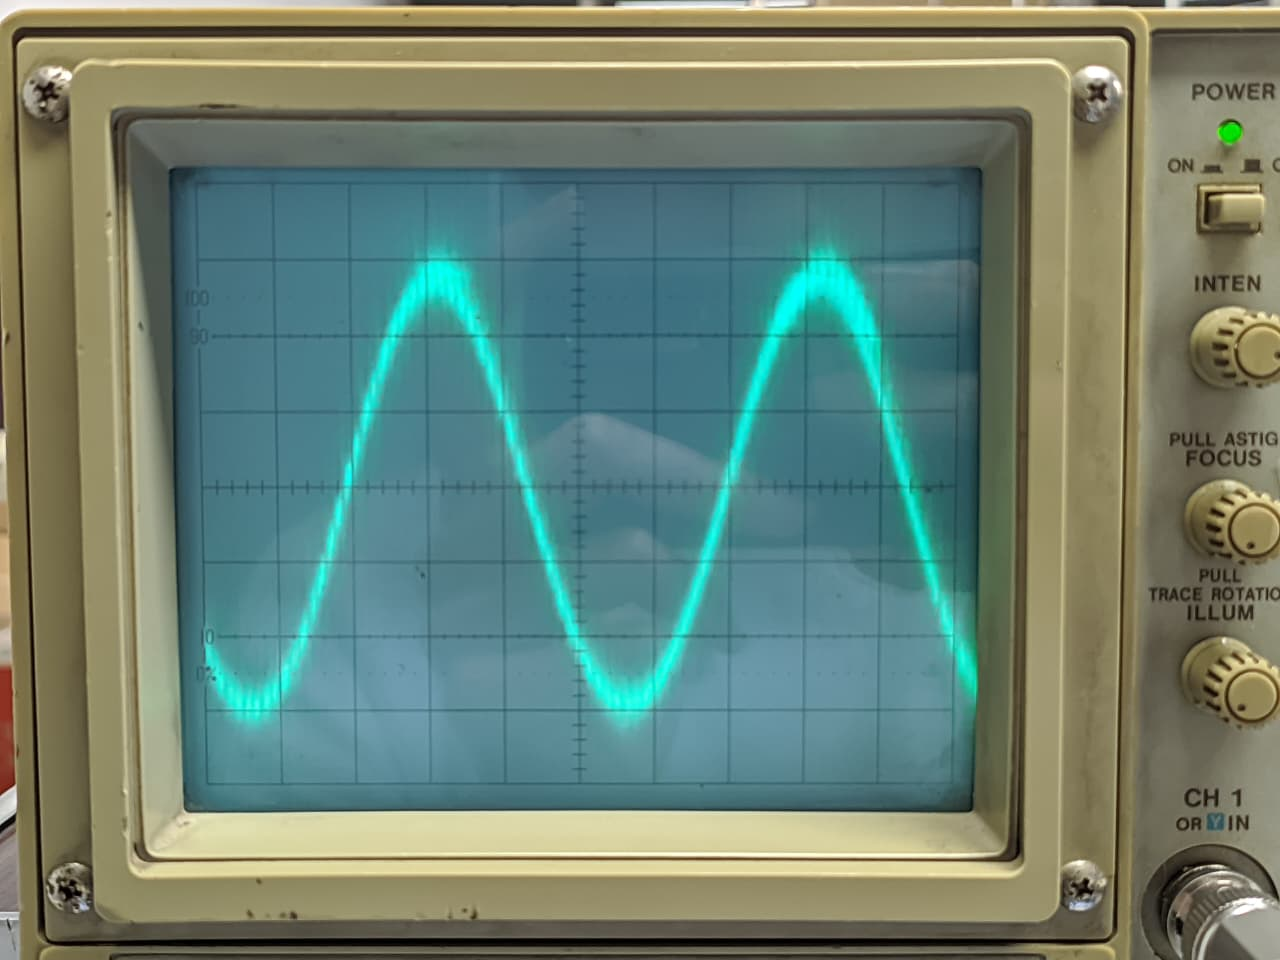
\includegraphics[height=0.35\textheight]{pictures/Medicion Vi.jpeg}
    \caption{$V_i$ en el osciloscopio. Escala: 1\,mV/div, 2\,ms/div.}
  \end{subfigure}
\end{figure}
\end{frame}


\begin{frame}{}

\begin{block}{Ganancia de tensión $A_v$}
\[
A_v = \frac{V_o}{V_i} = \frac{1\,\text{Vpp}}{6\,\text{mVpp}} \approx 166
\]
\end{block}

\begin{block}{Ganancia de corriente $A_i$}
\[
i_i = \frac{V_s - V_i}{R_s} = \frac{6\,\text{mVpp}}{6.8\,\Omega} \approx 0.88\,\text{mA}
\]
\[
i_o = \frac{V_o}{R_L} = \frac{1\,\text{Vpp}}{2.2\,\text{k}\Omega} \approx 0.4545\,\text{mA}
\]
\[
A_i = \frac{i_o}{i_i} = \frac{0.4545}{0.88} \approx 0.516
\]
\end{block}

\begin{block}{Impedancia de entrada $Z_i$}
\[
Z_i = \frac{V_i}{i_i} = \frac{6\,\text{mVpp}}{0.88\,\text{mA}} \approx 6.82\,\Omega
\]
\end{block}

\end{frame}



\begin{frame}{}

\begin{block}{Impedancia de salida $Z_o$}
\[
Z_o = \frac{V_o}{i_o}
\]
\[
i_o = \frac{V_o}{R_L} = \frac{1\,\text{Vpp}}{2.2\,\text{k}\Omega}
\]
\[
Z_o = \frac{1\,\text{Vpp}}{\tfrac{1\,\text{Vpp}}{2.2\,\text{k}\Omega}}
\]
\[
Z_o \approx 2.2\,\text{k}\Omega
\]
\end{block}

\end{frame}
